%% fcup-thesis.tex -- document template for PhD theses at FCUP
%%
%% Copyright (c) 2015 João Faria <joao.faria@astro.up.pt>
%%
%% This work may be distributed and/or modified under the conditions of
%% the LaTeX Project Public License, either version 1.3c of this license
%% or (at your option) any later version.
%% The latest version of this license is in
%%     http://www.latex-project.org/lppl.txt
%% and version 1.3c or later is part of all distributions of LaTeX
%% version 2005/12/01 or later.
%%
%% This work has the LPPL maintenance status "maintained".
%%
%% The Current Maintainer of this work is
%% João Faria <joao.faria@astro.up.pt>.
%%
%% This work consists of the files listed in the accompanying README.

%% SUMMARY OF FEATURES:
%%
%% All environments, commands, and options provided by the `ut-thesis'
%% class will be described below, at the point where they should appear
%% in the document.  See the file `ut-thesis.cls' for more details.
%%
%% To explicitly set the pagestyle of any blank page inserted with
%% \cleardoublepage, use one of \clearemptydoublepage,
%% \clearplaindoublepage, \clearthesisdoublepage, or
%% \clearstandarddoublepage (to use the style currently in effect).
%%
%% For single-spaced quotes or quotations, use the `longquote' and
%% `longquotation' environments.


%%%%%%%%%%%%         PREAMBLE         %%%%%%%%%%%%

%%  - Default settings format a final copy (single-sided, normal
%%    margins, one-and-a-half-spaced with single-spaced notes).
%%  - For a rough copy (double-sided, normal margins, double-spaced,
%%    with the word "DRAFT" printed at each corner of every page), use
%%    the `draft' option.
%%  - The default global line spacing can be changed with one of the
%%    options `singlespaced', `onehalfspaced', or `doublespaced'.
%%  - Footnotes and marginal notes are all single-spaced by default, but
%%    can be made to have the same spacing as the rest of the document
%%    by using the option `standardspacednotes'.
%%  - The size of the margins can be changed with one of the options:
%%     . `narrowmargins' (1 1/4" left, 3/4" others),
%%     . `normalmargins' (1 1/4" left, 1" others),
%%     . `widemargins' (1 1/4" all),
%%     . `extrawidemargins' (1 1/2" all).
%%  - The pagestyle of "cleared" pages (empty pages inserted in
%%    two-sided documents to put the next page on the right-hand side)
%%    can be set with one of the options `cleardoublepagestyleempty',
%%    `cleardoublepagestyleplain', or `cleardoublepagestylestandard'.
%%  - Any other standard option for the `report' document arclass can be
%%    used to override the default or draft settings (such as `10pt',
%%    `11pt', `12pt'), and standard LaTeX packages can be used to
%%    further customize the layout and/or formatting of the document.

%% *** Add any desired options. ***
%PDF
%\documentclass[a4paper,narrowmargins,11pt,oneside,draft,onehalfspaced,singlespacednotes]{fcup-thesis}
%\documentclass[a4paper,narrowmargins,11pt,oneside,onehalfspaced,singlespacednotes]{fcup-thesis}
%Print
%\documentclass[draft,a4paper,narrowmargins,11pt,twoside,openright,onehalfspaced,singlespacednotes]{fcup-thesis}
\documentclass[a4paper,narrowmargins,11pt,twoside,openright,onehalfspaced,singlespacednotes]{fcup-thesis}

%% *** Add \usepackage declarations here. ***
%% The standard packages `geometry' and `setspace' are already loaded by
%% `ut-thesis' -- see their documentation for details of the features
%% they provide.  In particular, you may use the \geometry command here
%% to adjust the margins if none of the ut-thesis options are suitable
%% (see the `geometry' package for details).  You may also use the
%% \setstretch command to set the line spacing to a value other than
%% single, one-and-a-half, or double spaced (see the `setspace' package
%% for details).
% Overfull statements
\pretolerance=150
\setlength{\emergencystretch}{3em}
% Overfull end
\usepackage[english]{babel}
\usepackage{helvet} %To replace arial fonts
\usepackage{lipsum}
\usepackage[utf8]{inputenc}


%%% Additional useful packages
%%% ----------------------------------------------------------------
\usepackage{array}
\usepackage{amsmath}  
\usepackage{amssymb}
\usepackage{amsfonts}
\DeclareFontFamily{OT1}{pzc}{}
\DeclareFontShape{OT1}{pzc}{m}{it}{<-> s * [0.900] pzcmi7t}{}
\DeclareMathAlphabet{\mathpzc}{OT1}{pzc}{m}{it}
%Titles need to be 14 pt => Large in \normaltext 11pt
\usepackage{titlesec}
\titleformat*{\section}{\Large\bfseries}
\titleformat*{\subsection}{\Large\bfseries}
\titleformat*{\subsubsection}{\Large\bfseries}
%Titles need to be 14 pt => Large in \normaltext 11pt
\usepackage{amsthm}      
\usepackage[ruled,algochapter]{algorithm2e}
\usepackage{algorithmic}
\usepackage{bm}
\usepackage[mathscr]{euscript}
\usepackage{graphicx}       
\usepackage{psfrag}         
\usepackage{fancyvrb}    
\usepackage{float}
\usepackage{ltablex}
\usepackage[square,sort,comma,numbers]{natbib}        
\usepackage{bbding}         
\usepackage{dcolumn}        
\usepackage{booktabs} 
\usepackage{multirow}
\usepackage{paralist}     
\usepackage{ifdraft}  
\usepackage{indentfirst}    
\usepackage[nottoc,notlof,notlot]{tocbibind}
\usepackage{url}
\usepackage{tabularx}
%use font size for captions like 8pt -> normalisize 11pt, scriptsize->8pt
\usepackage[font={scriptsize}]{caption}
\usepackage[font={scriptsize}]{subcaption}
\captionsetup{font=scriptsize}

\usepackage[unicode]{hyperref}
\usepackage{xcolor}


\hypersetup{pdftitle=Obstacle avoidance framework based on reach sets, 
            pdfauthor=Alojz Gomola,
            colorlinks=false,
            urlcolor=blue,
            pdfstartview=FitH,
            pdfpagemode=UseOutlines,
            pdfnewwindow,
            breaklinks
          }
\usepackage{array}
\newcolumntype{L}[1]{>{\raggedright\let\newline\\\arraybackslash\hspace{0pt}}m{#1}}
\newcolumntype{C}[1]{>{\centering\let\newline\\\arraybackslash\hspace{0pt}}m{#1}}
\newcolumntype{R}[1]{>{\raggedleft\let\newline\\\arraybackslash\hspace{0pt}}m{#1}}         
\newcolumntype{B}{X}
\newcolumntype{S}[1]{>{\hsize=#1\textwidth}X}

\newcommand{\FIGDIR}{./Pics}    %%% directory containing figures
\newcommand{\twolinecellr}[2][r]{%
  \begin{tabular}[#1]{@{}r@{}}#2\end{tabular}}
\newcommand{\secState}[1]{
	\ifdraft{(#1) }{}
}
\theoremstyle{plain}
\newtheorem{theorem}{Theorem}
\newtheorem{lemma}[theorem]{Lemma}
\newtheorem{proposition}[theorem]{Proposition}

\theoremstyle{plain}
\newtheorem{definition}{Definition}
\newtheorem{problem}{Problem}
\newtheorem{example}{Example}
\newtheorem{assumption}{Assumption}

\theoremstyle{remark}
\newtheorem*{corollary}{Corollary}
\newtheorem*{note}{Note}




\newenvironment{dokaz}{
  \par\medskip\noindent
  \textit{Proof}.
}{
\newline
\rightline{\SquareCastShadowBottomRight}
}

\newenvironment{constraints}[1]{
  \par\medskip\noindent
  \textit{Constraints #1} \\
}{
\newline
\rightline{\SquareCastShadowBottomRight}
}


%\bibliographystyle{plainnat}     %% Author (year) style
\bibliographystyle{unsrt}        %% [number] style
\setcitestyle{square}

% Section  3.7 Challenge list
\newif\ifproblemchallenge   %# Build block for problem challenges
\problemchallengetrue       %# Show comments

\newcommand{\R}{\mathbb{R}}
\newcommand{\N}{\mathbb{N}}

\DeclareMathOperator{\pr}{\textsf{P}}
\DeclareMathOperator{\E}{\textsf{E}\,}
\DeclareMathOperator{\var}{\textrm{var}}
\DeclareMathOperator{\sd}{\textrm{sd}}


\newcommand{\T}[1]{#1^\top}        

\newcommand{\goto}{\rightarrow}
\newcommand{\gotop}{\stackrel{P}{\longrightarrow}}
\newcommand{\maon}[1]{o(n^{#1})}
\newcommand{\abs}[1]{\left|{#1}\right|}
\newcommand{\dint}{\int_0^\tau\!\!\int_0^\tau}
\newcommand{\isqr}[1]{\frac{1}{\sqrt{#1}}}
\newcommand{\norm}[1]{\left\lVert#1\right\rVert}


\newcommand{\pulrad}[1]{\raisebox{1.5ex}[0pt]{#1}}
\newcommand{\mc}[1]{\multicolumn{1}{c}{#1}}
\newcommand{\TBD}[1]{\color{red}\emph{--TBD:}#1\color{black}}

%%%%%%%%%%%%%%%%%%%%%%%%%%%%%%%%%%%%%%%%%%%%%%%%%%%%%%%%%%%%%%%%%%%%%%%%
%%                                                                    %%
%%                   ***   I M P O R T A N T   ***                    %%
%%                                                                    %%
%%  Fill in the following fields with the required information:       %%
%%   - \degree{...}       name of the degree obtained                 %%
%%   - \department{...}   name of the graduate department             %%
%%   - \gradyear{...}     year of graduation                          %%
%%   - \author{...}       name of the author                          %%
%%   - \title{...}        title of the thesis                         %%
%%%%%%%%%%%%%%%%%%%%%%%%%%%%%%%%%%%%%%%%%%%%%%%%%%%%%%%%%%%%%%%%%%%%%%%%

%% *** Change this example to appropriate values. ***
\degree{Doctor of Philosophy}
\department{Departamento de Matem\'{a}tica}
\gradyear{2019}
\author{Alojz Gomola}
\title{Obstacle Avoidance Framework based on Reach Sets}

%% *** NOTE ***
%% Put here all other formatting commands that belong in the preamble.
%% In particular, you should put all of your \newcommand's,
%% \newenvironment's, \newtheorem's, etc. (in other words, all the
%% global definitions that you will need throughout your thesis) in a
%% separate file and use "\input{filename}" to input it here.


%% *** Adjust the following settings as desired. ***

%% List only down to subsections in the table of contents;
%% 0=chapter, 1=section, 2=subsection, 3=subsubsection, etc.
\setcounter{tocdepth}{3}

%% Make each page fill up the entire page.
\flushbottom


%%%%%%%%%%%%      MAIN  DOCUMENT      %%%%%%%%%%%%

\begin{document}



%%%%%%%%%%%%%%%%%%%%%%%%%%%%%%%%%%%%%%%%%%%%%%%%%%%%%%%%%%%%%%%%%%%%%%%%
%%  Put your Chapters here; the easiest way to do this is to keep     %%
%%  each chapter in a separate file and `\include' all the files.     %%
%%  Each chapter file should start with "\chapter{ChapterName}".      %%
%%  Note that using `\include' instead of `\input' will make each     %%
%%  chapter start on a new page, and allow you to format only parts   %%
%%  of your thesis at a time by using `\includeonly'.                 %%
%%%%%%%%%%%%%%%%%%%%%%%%%%%%%%%%%%%%%%%%%%%%%%%%%%%%%%%%%%%%%%%%%%%%%%%%

%% *** Include chapter files here. ***
\setcounter{chapter}{7}

%08-Conclusion
	\cleardoublepage
\chapter{\secState{R/W}Conclusion and Future Work}\label{ch:Conclusion}
\noindent This section summarizes \emph{obstacle avoidance framework} functionality (sec. \ref{s:conclusionSummary}), provides \emph{comparison to other methods} (sec. \ref{s:OtherMethodsComparison}), outlines \emph{approach reusability} (sec. \ref{s:approachReusability}), summarizes \emph{lessons learned} (sec. \ref{s:lessonsLearned}) and introduces possible \emph{future research heading} (sec. \ref{s:futureWork}).
	\section{\secState{R}Summary}\label{s:conclusionSummary}
\noindent The approach presented in (ch. \ref{ch:approach}) is covering the challenges (fig. \ref{fig:AvoidanceLevels}) related to:

\begin{enumerate}
    \item \emph{Reactive avoidance} - covering static obstacles, moving intruders, geo-fencing, weather effects.
    
    \item \emph{Event-based avoidance} - covers core UTM functionality and cooperative avoidance.
    
    \item \emph{Pre-emptive avoidance} - not covered in this work, the assumption about initial waypoint reachability still holds (ass. \ref{ass:reachableWaypoints}).
\end{enumerate}

\paragraph{Reactive Avoidance Test Coverage:} Testing avoidance capabilities against \emph{static obstacles}, \emph{non-cooperative intruders}, \emph{moving hard constraints} are covered. Coverage of the \emph{soft constraints}, \emph{map obstacles}, and \emph{detected obstacles} are implicitly covered due to the properties of \emph{safety} and \emph{body} margins (tab. \ref{tab:uncontrolledAirspaceViolations}).
    
\begin{enumerate}
    \item \emph{Building Avoidance} (sec. \ref{s:testBuildingAvoidance}) covers \emph{static obstacles} explicitly and \emph{map obstacles, hard constraints, ground avoidance} implicitly.
    
    \item \emph{Slalom} (sec. \ref{s:testSlalom}) covers \emph{open space navigation capabilities}, showing the determinism of the \emph{avoidance loop run}, in addition to \emph{building avoidance}.
    
    \item \emph{Maze} (sec. \ref{s:testMaze}) covers \emph{closed space navigation capabilities}, showing the higher level navigation properties of primitive \emph{right-side} 2D maze solver. The main point is to show possibility to enrich the \emph{Navigation loop algorithm} (fig. \ref{fig:missionControlRunActivityDiagram}).
    
    \item \emph{Storm} (sec. \ref{s:testStorm}) covers \emph{hard moving constraints avoidance} explicitly and \emph{hard static constraints}, \emph{soft static constraints}, \emph{soft moving constraints} implicitly.
    
    \item \emph{Emergency converging} scenario (sec. \ref{s:testEmergencyConverging}) covers \emph{non-cooperative intruder with the right of the way} avoidance capability.
    
    \item \emph{Emergency head-on} scenario covers (sec. \ref{s:testEmergencyHeadOn}) \emph{non-cooperative intruder without right of the way} avoidance capability
    
    \item \emph{Emergency mixed} scenario (sec. \ref{s:testEmergencyMixed}) covers \emph{multiple intruders with/without right of the way} avoidance capability.
\end{enumerate}

\paragraph{Event-Based Avoidance Coverage:} Test cases covers \emph{well clear breach prevention}, \emph{situation-based avoidance}, and \emph{rules of the air enforcement}. Coverage of \emph{near miss situations}, \emph{clash incidents} is given implicitly by \emph{safety} and \emph{body} margins (tab. \ref{tab:controlledAirspaceViolations}).

\begin{enumerate}
    \item \emph{Rule-based converging} (sec. \ref{s:testRuleConverging}) covers \emph{well clear breach} and \emph{the converging rule of the air}, showing determinism and \emph{UTM resolution execution}.
    
    \item \emph{Rule-based head-on} (sec. \ref{s:testRuleHeadOn}) covers \emph{well clear breach} and \emph{head on rule of the air}, showing determinism and \emph{UTM resolution execution}.
    
    \item \emph{Rule-based mixed head on with converging} (sec. \ref{s:testRuleMixed}) covers \emph{well clear breach} and \emph{head on and converging rules of the air}. The main focus is on the \emph{virtual roundabout} concept when multiple collision cases are clustered into one avoidance maneuver. 
    
    \item \emph{Rule-based overtake} (sec. \ref{s:testRuleOvertake}) covers \emph{well clear breach} during \emph{overtaking} by faster UAS.
\end{enumerate}


\subsection{\secState{R} Hierarchical Decision Making}\label{s:conclusionAvoidanceNavigationRun}
\noindent The key feature of the approach is hierarchical decision making. The hierarchy is introduced not only to threat prioritization but also to the time sequence of the decisions. The framework scheme (fig. \ref{fig:AvoidanceFrameworkConceptNew}) shows that situational assessment in the form of \emph{data fusion} is done in (sec. \ref{s:sensorFusion}). The trajectory selection process is separated from the final avoidance strategy pick-up process. The decision making separation is done like follows:

\begin{itemize}
    \item[$\to$] \emph{Avoidance Run} (sec. \ref{s:aviudabceGridRun}) - for one specific data set, for a fixed time, for a fixed goal find the cheapest trajectory which is safe (reachable).
    
    \item[$\to$] \emph{Navigation Run} (sec. \ref{s:missionControlRun}) - for multiple data sets (threat hierarchy), for a fixed time, for context depending goal try to find existing solution as a safe trajectory. Select trajectory breaking least restrictions from candidates.
\end{itemize}

The decision making process on threat assessment level (fig. \ref{fig:missionControlRunActivityDiagram}) is the configuration of threat type application in 7\textsuperscript{th}-10\textsuperscript{th} step. The idea is that UAS:
\begin{enumerate}
    \item must avoid any \emph{static obstacles} (sec. \ref{s:detectedObstacles}),
    
    \item can skip \emph{intruders} (sec. \ref{s:intruders}) if there are no other options
    
    \item can enter into \emph{hard constraints} (sec. \ref{s:virtualConstraints}, def. \ref{def:movingConstraint}) area if its necessary,
    
    \item can enter into \emph{soft constraints} (sec. \ref{s:virtualConstraints}, def. \ref{def:movingConstraint}) area if its necessary.
\end{enumerate}

\begin{note}
    The \emph{implementation} of \emph{soft/hard constraints} and their evaluation process is same in \emph{avoidance run}; the only difference is when they are applied by \emph{navigation run}.
\end{note}
    
\subsection{\secState{R}Use of Developed Reach Set Approximations}\label{s:conclusionReachSet}

\noindent The reach set approximation (sec. \ref{s:reachSet}) represents a set of  \emph{maneuvering} strategies (avoidance/movement) which can be used in a different context. The properties of the trajectories are given based on \emph{constrained expansion} (sec. \ref{s:constrainedTrajectoryExpansion}) and performance parameters priority (sec. \ref{s:ReachSetPerformanceCriteria}).

The conditions and priorities are changing with the operational environment, to successful integration into nonsegregated airspace is necessary to reflect this.  For this purpose, the multiple reach set approximation approaches were developed. The performance tests and longer summary can be found in (sec. \ref{sec:reducedReachSetPerformance}). The summary of each reach set approximation method is given like follow:

\begin{itemize}
    \item[$\to$] \emph{Chaotic reach set approximation} (sec. \ref{s:chaoticReachSet}) - contains a lot of \emph{curved trajectories} with high space coverage ratio, used for \emph{emergency reactive avoidance} in non-controlled/controlled airspace, \emph{last resort reach set}.
    
    \item[$\to$] \emph{Harmonic reach set approximation} (sec. \ref{s:harmonicReachSet}) -  contains a lot of \emph{straight} trajectories with low space coverage ratio, used for navigation in \emph{non-controller airspace}.
    
    \item[$\to$] \emph{Combined reach set approximation} (sec. \ref{s:combinedReachSet}) - the reach set approximation is represented as a tree, there is a possibility to combine two or more reach sets with the same initial state, the outcome of such merge is a new reach state with different properties.
    
    \item[$\to$] \emph{ACAS-like reach set approximation} (sec. \ref{s:acasReachSet}) - contains \emph{mandatory separations} (depending on aircraft type), has low trajectory count and low coverage ratio, it emulates ACAS maneuver table in reach set data structure, used for navigation and avoidance in ATC controlled airspace.
\end{itemize}
	\newpage
\section{Comparison to Other Methods}\label{s:OtherMethodsComparison}
\noindent The \emph{testing} (sec. \ref{s:testPlan}) is strongly \emph{capability} oriented, some performance testing regrading computational load (sec. \ref{s:ComputaitonFootprint}) is on the place. The advantages of our approach regarding scalability are outlined in (sec. \ref{s:conclusionScalability}).

This section summarizes the results achieved by one of the master students \cite{hrdlik2018}. Who compares other avoidance methods concerning performance. The  \emph{conservative }vector field avoidance \cite{borenstein1991vector} and \emph{adaptive} potential field \cite{koren1991potential} methods are compared to our approach (sec. \ref{s:conservativeComparison}).

\subsection{Conservative and Adaptive Method Comparison}\label{s:conservativeComparison}
\paragraph{Testing scenario:} The testing scenario is similar to \emph{building avoidance} (sec. \ref{s:testBuildingAvoidance}), using the default framework testing configuration (sec. \ref{sec:testingConfiguration}). The \emph{reach set approximation} used is a \emph{combination of TM-RSA and CM-RSA} (fig. \ref{fig:combinedReachSetApproximation}) filling the role for \emph{navigation/avoidance} in non controlled airspace. The \emph{mission} is given by waypoints defined in (tab. \ref{tab:missionSetupForPErformanceTest}), the UAS is starting at $\mathscr{WP}_1$.

\begin{table}[H]
	\centering
	\begin{tabular}{c|c||c|c|c|c|c}
		\multicolumn{2}{c||}{Position} & \multicolumn{4}{c}{Waypoints} \\\hline
		$[x,y,z]$     & $[\theta,\varpi,\psi]$           & $\mathscr{WP}_1$   & $\mathscr{WP}_2$   & $\mathscr{WP}_3$   & $\mathscr{WP}_4$    & $\mathscr{WP}_5$\\\hline\hline
		$[0,0,0]^T $       & $[0^\circ,0^\circ,0^\circ]^T$ & $[0,0,0]^T$ & $[20,0,0]^T$       & $[20,20,0]^T$       & $[0,20,0]^T$       & $[0,0,10]^T$       
	\end{tabular}
	\caption{Mission setup for \emph{Performance test} scenario.}
	\label{tab:missionSetupForPErformanceTest}
\end{table}

\noindent The \emph{static obstacle set} (tab. \ref{tab:obstacleSetComparison}) contains three obstacles in the middle of waypoints. The obstacles are balls with uniform radius. The concept of \emph{body} and \emph{safety margin} was not used in this test.

\begin{table}[H]
	\centering
	\begin{tabular}{c|c|c|c}
		\multicolumn{3}{c|}{Obstacle} &  \multirow{2}{*}{Radius}\\\cline{1-3}
		id & position & type  &   \\\hline\hline
		$1$ & $[10,0,0]^T$ & ball  &$2$ \\\hline
		$2$ & $[20,10,0]^T$ & ball & $2$ \\\hline 
		$3$ & $[10,20,0]^T$ & ball  & $2$ 
	 \end{tabular}
	\caption{\emph{Obstacle set} for \emph{Building avoidance} scenario.}
	\label{tab:obstacleSetComparison}
\end{table}

\begin{note}
The z coordinate value of zero does not represent the ground in this test scenario, because some methods do not support ground avoidance like ours. 
\end{note}

\paragraph{Scenario example:} The \emph{scenario} was run for the following approaches:
\begin{enumerate}
    \item \emph{Static obstacle avoidance based on reach sets} - implementation \cite{hrdlik2018} of \cite{gomola2017obstacle}, using own framework.
    
    \item \emph{Conservative } - vector field avoidance \cite{borenstein1991vector}, adapted implementation \cite{hrdlik2018}.
    
    \item \emph{Adaptive} - potential field \cite{koren1991potential}, adapted implementation \cite{hrdlik2018}.
\end{enumerate}

\noindent The example of the testing framework developed by my student is shown in (fig. \ref{fig:avoidancePerformanceScenarioHrdlik}). The \emph{obstacles} are big red balls consisting from smaller red balls, representing LiDAR sensor hit zones. The \emph{UAS} sensing range is represented as an area outlined with a black dashed line. The waypoints are marked as green squares. The flew trajectory is represented as blue line. The \emph{planned trajectories} (red line) for decision frames (magenta circle) which are not executed are also shown.

\begin{figure}[H]
    \centering
    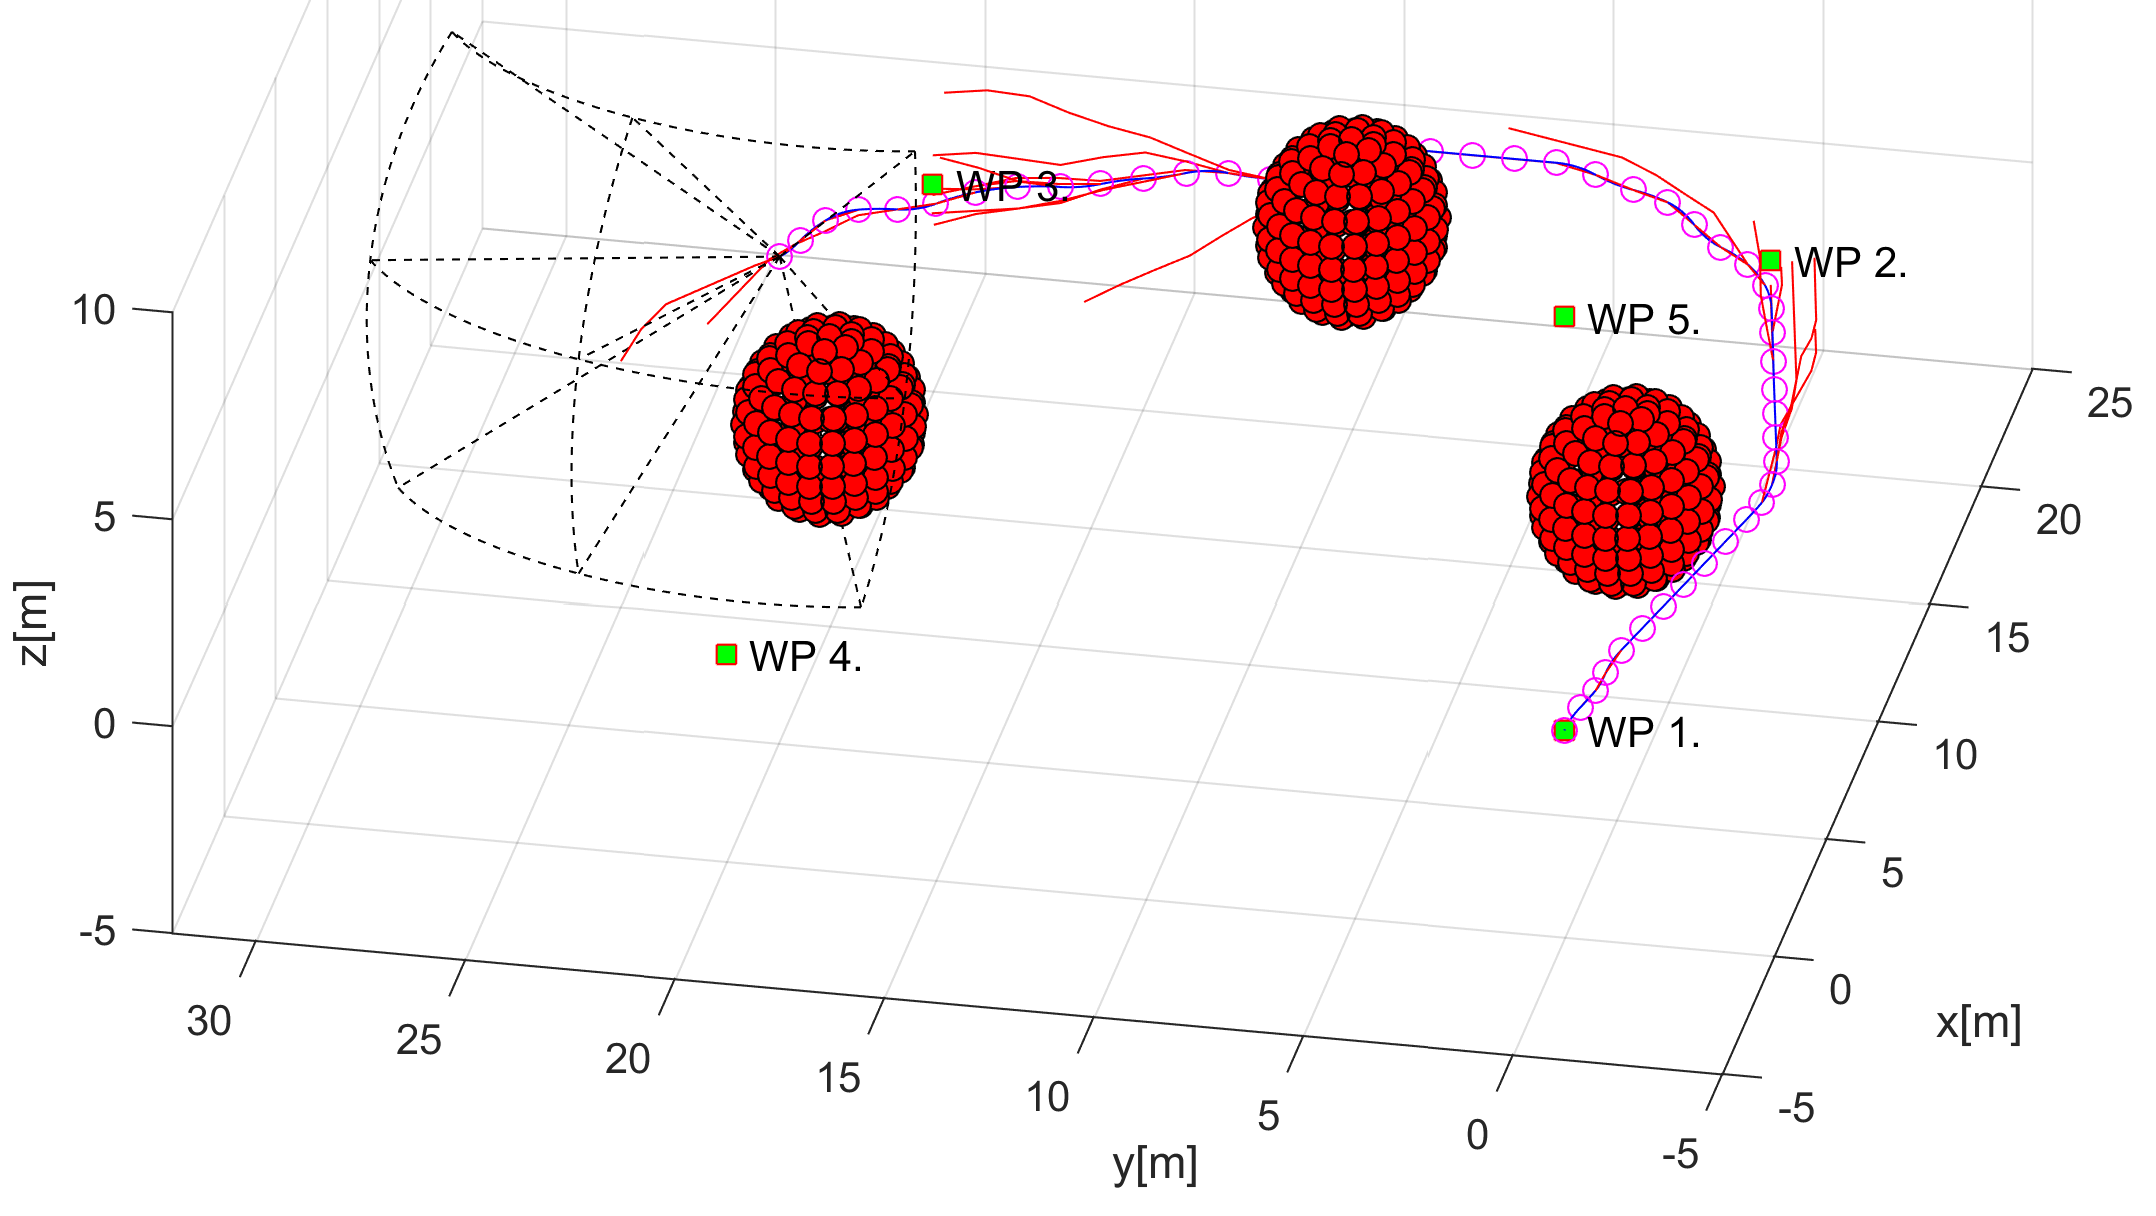
\includegraphics[width=0.7\linewidth]{\FIGDIR/C001TestingScenario} 
    \caption{A testing scenario for method performance comparison \cite{hrdlik2018}.}
    \label{fig:avoidancePerformanceScenarioHrdlik}
\end{figure}

\paragraph{Conservative Method Performance Margin:} The \emph{principle} of the conservative method is like follows: \emph{Every time there must be a place to turn without the context}. The conservative method performance margin was estimated by \cite{hrdlik2018} like follow:

\begin{equation*}
    conservative_{margin} = 2 \times turning Radius +3 \times uas Radius
\end{equation*}

\noindent Using parameters from our testing configuration (sec. \ref{sec:testingConfiguration}) where the turning radius is 2 and UAS body radius is 0.6 the theoretical $conservative_{margin}$ is $4.6$.

\paragraph{Conservative Method Performance Margin:} The \emph{principle} of the conservative method is like follows: \emph{Every mass point has a potential equal to its expected mass, those potentials repel each other with proportional force}. The adaptive method performance margin was estimated by \cite{hrdlik2018} like follow:

\begin{equation*}
    adaptive_{margin} = 3\times uas Radius
\end{equation*}

\noindent Using parameters from our testing configuration (sec. \ref{sec:testingConfiguration}) where the UAS body radius is 0.6 the theoretical $adaptive_{margin}$ is $1.8$.

\begin{note}
    The \emph{real conservative and method performance}  was close to \emph{theoretical best performance} \cite{hrdlik2018}.
\end{note}

\paragraph{Distance to Body Margin Evolution:} The performance of an \emph{obstacle avoidance framework based on reach set} for the mission (tab. \ref{tab:missionSetupForPErformanceTest}) is shown in (fig. \ref{fig:crashDistanceEvolution}). The critical margin (crash zone) is 0.6 (UAS body radius) and is denoted as a red dashed line. The \emph{adaptive margin} id 1.8 and its denoted as a yellow dashed line. The \emph{conservative margin} is 4.6 and its denoted as green dashed line. 

The distance to the \emph{body margin} of the UAS center stayed mostly in \emph{adaptive zone} (yellow line) and two times entered into \emph{outperforming zone} (red line). The \emph{outperforming zone} is distance values between:

\begin{equation*}
    critical Margin (0.6) \ge outperforming Zone < adaptive Margin (1.8)   
\end{equation*}

One can say that reach set method outperforms selected conservative and adaptive methods representatives.

\begin{figure}[H]
    \centering
    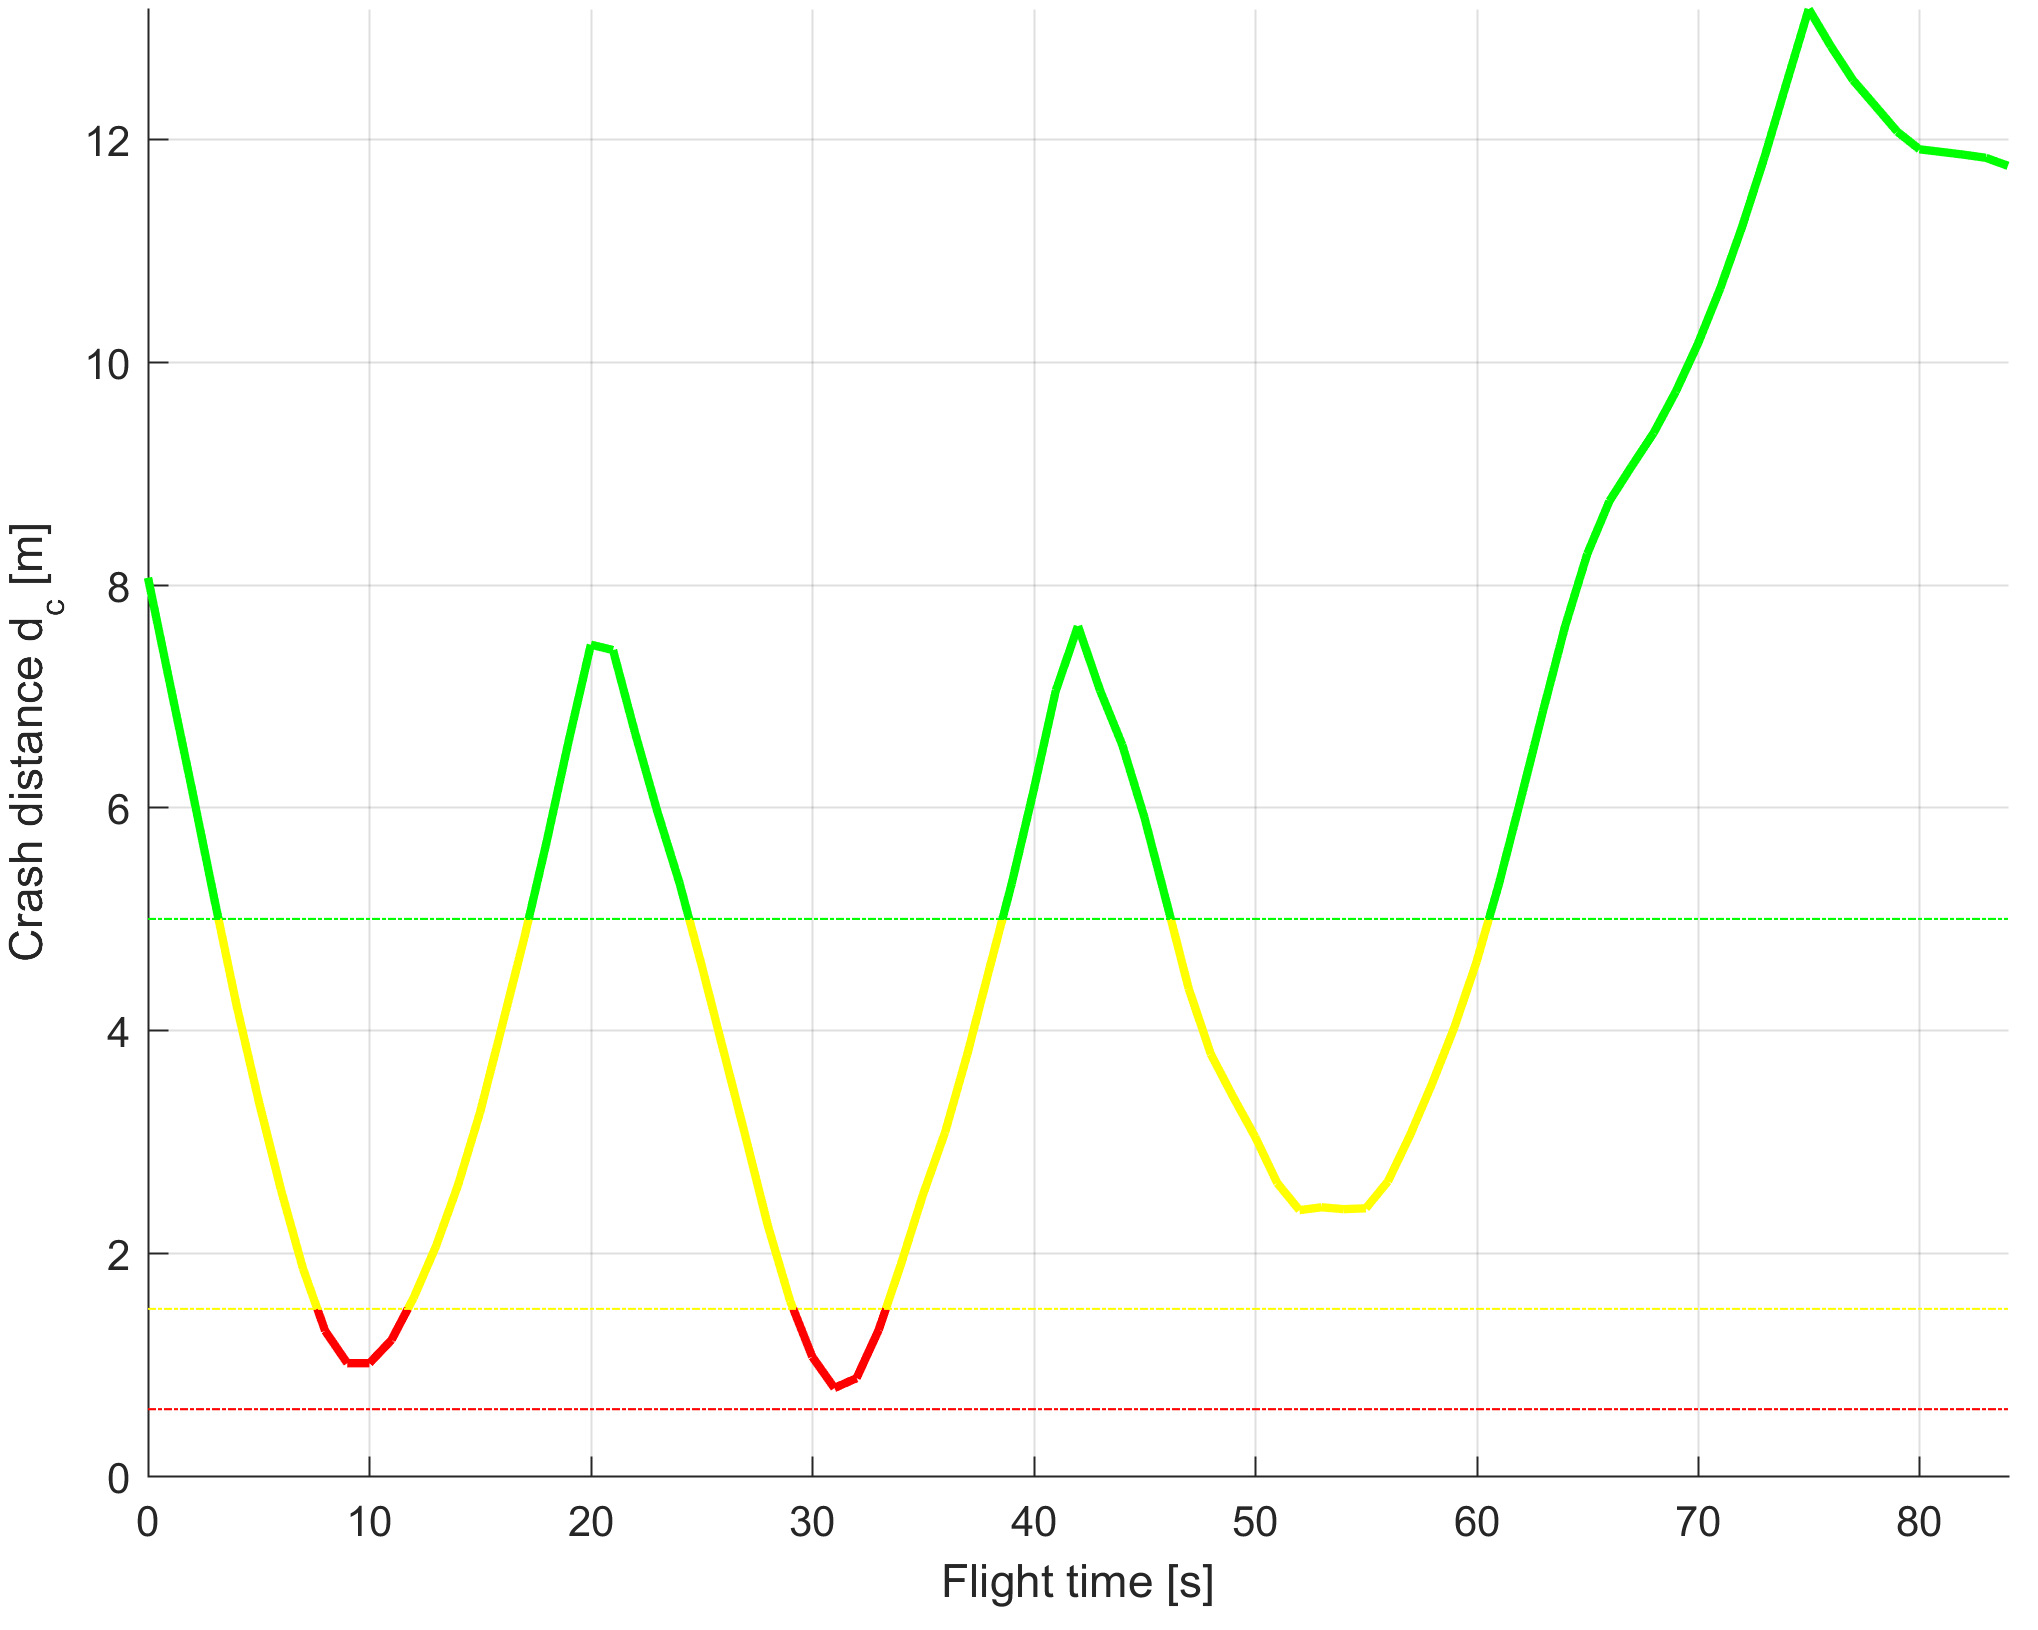
\includegraphics[width=0.7\linewidth]{\FIGDIR/C002CrashDistanceEvolution} 
    \caption{Distance to body margin evolution \cite{hrdlik2018}.}
    \label{fig:crashDistanceEvolution}
\end{figure}

\paragraph{Disclaimer:} Further investigation regarding \emph{cost-effectiveness} is required, the approach needs to be tested in real environment and on the multiple scenarios. The testing concerning approach feasibility have been proven (tab. \ref{tab:testCasesPerformacneEvaluation}).

\subsection{Scalability}\label{s:conclusionScalability}
\noindent The \emph{many methods} do not offer \emph{scalability}. The scalability means that method applies to multiple problems with different scale or there is a sufficient amount of tune-able parameter to make it work in different environments. Many avoidance concepts have hardwired margins. 

The \emph{Detect and Avoid} system must offer scalability to some extent, because of changing regulations and performance criteria on the UAS systems.

\paragraph{Range scalability:} The physical constraints need to be sensed by sensor array in avoidance grid, and the UAS cannot get to close to them. 

\paragraph{Static obstacles:} The body margin or the minimal distance of UAS center to obstacle body is constrained like follow:

\begin{equation*}
    uas Radius < body Margin \le grid Range
\end{equation*}

The \emph{tuning parameter} for static obstacles is \emph{safety margin} is then constrained like follow:

\begin{equation*}
    body Margin < safety Margin \le \infty
\end{equation*}


The constraints for safety margin calculation and some guidelines were outlined in (app. \ref{s:safetyMarginCalculation}).

\paragraph{Intruders:} The \emph{intruders} (sec. \ref{s:intruders}) are limited by \emph{detection range} and intersection models parameters ranges. 

The \emph{body volume intersection} (app. \ref{s:bodyvolumeIntersection}) has a following constraint:

\begin{equation*}
    intruder Radius < body Radius \le minimal Detection Range - 2 \times our UAS radius
\end{equation*}

\begin{note}
    The \emph{body radius} does not need to fit exactly on the intruder real body radius; usually, some padding space is added.
\end{note}

The \emph{maneuverability uncertainty intersection} (app. \ref{s:uncertaintyIntersection}) is tuned through the uncertainty spread on the horizontal and vertical plane. This spread cannot be infinite, and the only limitation is given by implementation:

\begin{equation*}
    \begin{aligned}
        0^\circ & \le&  horizontal Spread &< &90^\circ\\
        0^\circ & \le&  vertical Spread &< &90^\circ
    \end{aligned}
\end{equation*}



\paragraph{Constraints:} The constraints are considered as \emph{airspace restrictions}, \emph{weather zones}, \emph{geo-fencing zones} in this work. The constraints have two implementations \emph{Static constraints} (sec. \ref{s:virtualConstraints}) and \emph{Moving constraints} (def. \ref{def:movingConstraint}). The only real constraint is the detection range; the constraint must be detected before making any impact on \emph{grid}:

\begin{equation*}
    impact(uasPosition,constraintCenter) < detection Range - grid Range
\end{equation*}




	\section{\secState{R}Approach Reusability}\label{s:approachReusability}
\noindent The  \emph{avoidance framework} can be used as a whole, or some of the concepts can be transferred as modules to other approaches. This section picks such reusable concepts,

\paragraph{UTM Services:} The constrained \emph{UTM functionality} is outlined in (sec. \ref{sec:UASTrafficManagement}) including:
\begin{enumerate}
    \item \emph{Future UTM Communication Architecture} (fig. \ref{fig:UTMArchitectureOverview}) as the authority over \emph{airspace segment} (fig. \ref{fig:DAMExample})\cite{gerdes2016dynamic}.
    
    \item \emph{Cooperative Conflict Resolution Under UTM Supervision} (fig. \ref{fig:CooperativeConflictResolutionUTM}) designed as mild/feasible directives (commands) with \emph{constant supervision}.
    
    \item \emph{Rules of the Air Enforcement} (sec. \ref{sec:handlingHeadOnApproach}, \ref{sec:handlingConvergingManuever}, \ref{sec:handlingOvertakeManuever}) including designs of \emph{Position Notification} (sec. \ref{sec:positionNotification}) and \emph{Collision Case Structure/Calculation} (sec. \ref{sec:collisionCase}).
    
    \item \emph{Divergence/Convergence Waypoints} concept is showcased in \emph{Overtake Rule} (rule \ref{tab:ruleOvertakeDefinition}). 
    
    \item \emph{Weather Avoidance} (app. \ref{sec:weatherCase}) is using a similar concept to \emph{Collision Case}: \emph{Weather Case}. The information is provided by \emph{Local Airspace Authority}.
    
\end{enumerate}

\paragraph{Emergency Avoidance Functionality:}  The standard framework implementation (fig. \ref{fig:missionControlRunActivityDiagram}) can handle the situations given in non-cooperative test cases (sec. \ref{s:noncooperativeTestCases}). The list of threats is given by (tab. \ref{tab:uncontrolledAirspaceViolations}). 

\paragraph{Event-Based Avoidance Functionality:} The standard framework implementation (fig. \ref{fig:missionControlRunActivityDiagram}) with active $C2$ link and rules setup (fig. \ref{fig:RuleEngineInstanceLevels}) can handle the situations given in cooperative test cases (\ref{s:cooperativeTestCases}). The list of threats is given by (tab. \ref{tab:controlledAirspaceViolations}). The \emph{Avoidance Mode Concept} enables to switch between \emph{Event-Based Avoidance} (Navigation) and \emph{Emergency Avoidance.}
\begin{note}
    The emergency Avoidance Functionality is included in \emph{Event-Based Avoidance} (Navigation) mode.
    The prioritization of \emph{threats} may differ (tab. \ref{tab:controlledAirspaceViolations}).
\end{note}

\paragraph{Reusability for More Complex Systems:} The framework (fig. \ref{fig:avoidanceConcept}) with implemented rule engine (fig. \ref{fig:RuleEngineBasicArchitecture}) can be used on \emph{any system}, with appropriate \emph{Movement automaton} (sec. \ref{s:segmentedMovementAutomaton}) enabling \emph{wave-front} propagation (alg. \ref{alg:Wavefront Propagation}) for reach set estimation. Following artifacts needs to be delivered for concept reuse:

\begin{enumerate}
    \item The \emph{Movement Automaton} is used to generate \emph{thick series of waypoints} which guarantees desired degree of safety.
    
    \item The \emph{complex UAS system} is following the \emph{reference trajectory} (sec. \ref{s:referenceTrajectoryGenerator}).
    
    \item The \emph{Sensor Fusion} (sec. \ref{s:SensorFusionDefinition}) implementation including classification to \emph{Free}, \emph{Occupied}, \emph{Restricted} space type.
    
    \item The \emph{sensor field} is supporting detection of threats. There should be at least one sensor with the capability of feeding \emph{Avoidance Grid}. Our implementation was based on LiDAR/ADS-B feeds.
    
    \item The \emph{Information Sources} are supporting the online/offline threat processing. This one is completely optional.
\end{enumerate}

\begin{note}
    \emph{On UTM integration:} The future UTM system will not be giving the extreme commands, the directives are more like constraints; therefore our system can provide the guidance and constraint evaluation
\end{note}

\begin{note}
    \emph{On Safety Margin:} The disparity between real flown trajectory (nonlinear dynamics) and planned trajectory (Movement Automaton) needs to be accounted into \emph{Safety Margin}.
\end{note}

\paragraph{Reach Set Approximations:} The \emph{wave-front} approach (alg. \ref{alg:Wavefront Propagation}) can be used with \emph{Constrained expansion function} (sec. \ref{s:constrainedTrajectoryExpansion}) to create own \emph{Reach set Approximation Method}. Existing  reach set approximation methods are always following a different goal; they can be reused for other tasks (perf. \ref{sec:reducedReachSetPerformance}):

\begin{enumerate}
    \item \emph{Chaotic} (def. \ref{s:chaoticReachSet}) - high space coverage, ideal for unpredictable and complex avoidance maneuvers.
    
    \item \emph{Harmonic} (def. \ref{s:harmonicReachSet}) - smooth trajectories, medium space coverage, ideal for navigation maneuvers.
    
    \item \emph{Combined} (def. \ref{s:combinedReachSet}) - a combination of the \emph{harmonic} and \emph{chaotic} approximations, the cost function defines preferred trajectories. The procedure is reusable for any reach set approximation types ($2^+$) combination.
    
    \item \emph{ACAS-X Like} (def. \ref{s:acasReachSet}) - following \emph{TCAS/ACAS separation modes}, can be used as an alternative for \emph{controlled avoidance} and \emph{navigation}.
\end{enumerate}
	\section{\secState{R}Lessons Learned}\label{s:lessonsLearned}
\noindent During the approach development, some mistakes were made. This section summarizes the most notable design choices with the reasoning behind them.

\paragraph{Euclidean vs. Planar Space Partitioning:} The \emph{operational space discretization} was planned from the beginning. The initial approach was to use a \emph{uniform Euclidean  grid} where the smallest space portion was represented as cubic cell.

\paragraph{Euclidean grid shortcomings:} The problem was with \emph{LiDAR} reading assessment because for each point it was necessary to do \emph{transformation} defined as  a series of the functions (eq. \ref{eq:cpt01}, \ref{eq:cpt02}, \ref{eq:cpt03}, \ref{eq:cpt04}). The continuous updating of the \emph{space assessment} usually timed-out. 

The other issue was with wavefront algorithm (alg. \ref{alg:Wavefront Propagation}). The intersection (def. \ref{def:ContainedReducedReachSet}) function was not problematic, due the unlimited estimation time of \emph{reach set approximation}. The \emph{reach set approximation} is shaped usually like the cone; therefore each propagation caused hitting more cells in Euclidean  grid. This caused the following challenges:

\begin{enumerate}
    \item \emph{An exponential growth of trajectory count} - the \emph{trajectory footprint} (def. \ref{def:trajectoryFootprint}) is almost always unique in Euclidean Grid. The problem is that two very similar trajectories concerning avoidance were considered unique.
    
    \item \emph{Low avoidance strategies variability} - the generated trajectories by \emph{harmonic} (sec. \ref{s:harmonicReachSet}) or \emph{chaotic} (sec. \ref{s:chaoticReachSet}) reach set approximation did not follow the desired properties of coverage.
    
    \item \emph{Threat impact reflection} - the space which is closer to UAS needs to be surveillance with greater detail than space which is further away from UAS. The Euclidean grid does not reflect this.
\end{enumerate}

\paragraph{Euclidean Grid Benefits:} The intersection model performance was good because of most of the numeric/analytically intersection solutions for:
\begin{enumerate}
    \item \emph{Line} - used in \emph{linear intruder intersection model} (sec. \ref{s:linearIntersectionModel}).
    
    \item \emph{Tunnel} - used in \emph{body-volume intersection model} (sec. \ref{s:bodyvolumeIntersection}).
    
    \item \emph{Polygon} - used in constraints (sec. \ref{s:virtualConstraints}, \ref{s:MovingVirtualConstraints})
\end{enumerate}

\paragraph{Planar Grid Deployment:} The shortcomings and benefits of \emph{Euclidean grid} are obvious, the main reason why the \emph{planar gird} was employed is the \emph{performance of the wave-front algorithm} (alg. \ref{alg:Wavefront Propagation}) for UAS system dynamic. The main focus of this work lies on \emph{Reach Set} properties, the planar grid (fig. \ref{fig:LidarSpaceSegmentation}) properties:

\begin{equation*}
    \uparrow distance \implies \uparrow cell Size \implies \downarrow importance
\end{equation*}

\noindent are ideal for \emph{avoidance problems}. The cell size is increasing proportionally with increasing distance. The space partitioning at the lower distance is dense, reflecting the importance of proximity threats. The space partitioning at the greater distance is getting looser, reflecting the unimportant of threats at greater distance. 

\noindent The \emph{planar grid} employment has following benefits:
\begin{enumerate}
    \item Fast \emph{LiDAR} (and other ranging sensors) clustering.
    \item Reflection of space importance.
    \item A significant increase of \emph{wave-front} algorithm.
    \item A significant decrease in reach set approximation node count.
\end{enumerate}

\noindent The \emph{planar grid} employment has the following shortcomings:
\begin{enumerate}
    \item Implementation complexity of intruder intersection models.
    \item Implementation complexity of constraints intersection models.
\end{enumerate}

\begin{note}
    The count of intruder and constraints is not so great concerning \emph{aerial transpiration}; the situation is opposite in case of \emph{ground transportation} especially road vehicles. 
\end{note}

\paragraph{Intruder Intersection Models:} The \emph{implemented intruder intersection models} (sec. \ref{s:intruderBehaviourPrediction}) are basic and sufficient. There are few ideas which do not make it into the final concept:

\begin{enumerate}
    \item \emph{Intruder as line/curve intersection} - the idea is to use a parametric curve instead of the \emph{linear intersection model} (sec. \ref{s:linearIntersectionModel}). The problem is those curve parameters are hard to obtain; they are not mandatory part of any position notification proposal so far.
	
	\item \emph{Intruder as movement automaton simulated trajectory} - the idea is to have access to movement automaton of an intruder in \emph{predictor mode} (sec. \ref{s:referenceTrajectoryGenerator}) to generate future expected trajectory. The problem is in some situations the trajectory of intruder changes a lot and \emph{maneuverability uncertainty intersection} (sec. \ref{s:uncertaintyIntersection}) outperforms this approach significantly. The other problem is that most of the \emph{general aviation} does not want to share this kind of information due to security reasons.  This concept makes it into the final solution, but not in \emph{avoidance framework}, but as \emph{UTM collision case intersection calculation} (sec. \ref{sec:collisionCase}).
	
	\item \emph{Intruder well clear implementation as a rule} - the idea is to implement \emph{potential fields principle} as core mechanism of avoidance. The problem is determinism of this approach, and the idea was scrapped.
\end{enumerate}

\paragraph{Approach to data fusion:} To make our approach universal, the decision to use input/output interfaces were made (fig. \ref{fig:AvoidanceFrameworkConceptNew}). The choice of the \emph{output control interface} is clear, the movement automaton (sec. \ref{sec:MovementAutomatonBackground}) was performing well from the beginning \cite{gomola2017optimal,gomola2017mpc}.

The \emph{input interface} represented as \emph{data fusion} (theory sec. \ref{s:dataFusionDefinition}, implementation sec \ref{s:sensorFusion}), was more problematic.

\paragraph{Deterministic approach:} The article \cite{gomola2017obstacle} and technical reports \cite{gomola2017mpc,gomola2017optimal} are using a deterministic approach where the property of the avoidance grid cell is given as a Boolean value. This approach is too restrictive because all the values needed to be determined on the spot. The overall data fusion was nonexistent because the approaches were used only static obstacles and \emph{LiDAR} sensor as the base. 

\paragraph{Probabilistic approach:} The technical report \cite{gomola2017probabilistic} introduced the \emph{intruders} and \emph{map obstacles} \cite{cernamaria2018}. This requires\emph{probabilistic implementation}. The probabilistic density functions with all that theoretical apparatus are established in order to cover the processes of the data fusion and decision making. The problem was the formalization level; much \emph{effort} is wasted to formalize very simple calculations and thresholds. The tuning parameters were nonexistent, preventing the customization.

\paragraph{Final Approach as a Synthesis:} The benefits of both approaches for data fusion are used in final implementation (sec. \ref{s:sensorFusion}), the useful aspects of probabilistic approach like ratings and addition rules persisted. The useful aspects of deterministic, like threshold, is kept through predicates (tab. \ref{tab:defuzificationRatings}). The concept is the following:

\begin{enumerate}
        \item \emph{Ratings reflects probabilities} - the property of visibility (eq. \ref{eq:visibilityForCell}), obstacle encounter in cell (eq. \ref{eq:detectedObstacleRatingForCell}), map obstacle in cell (eq. \ref{eq:mapObstacleRatingForCell}), intruder intersection with cell (eq. \ref{eq:intruderRatingForCell}), constraint intersection of the cell (eq. \ref{eq:constraintRatingForCell}) are formalized as threat property (def. \ref{def:threat}). 
	    
	    \item \emph{Man-made rules incorporation} - man-made rules can be incorporated into any part of the data fusion process.
	    
	    \item \emph{Situation assessment} - the known world classification through data fusion (eq. \ref{eq:UncertainDataFusion}) is implemented as cell set classification:
	    \begin{enumerate}[a.]
	        \item \emph{Uncertain} (eq. \ref{eq:UncertainDataFusion}) - the state of this space cannot be determined by sensors or prior knowledge.
	        
	        \item \emph{Occupied} (eq. \ref{eq:ocuupiedDataFusion}) -  these cells are occupied by a physical object, entering into this space will cause real damage to UAS.
	        
 	        \item \emph{Constrained} (eq. \ref{eq:constrainedDataFusion}) - intruder or other kinds of threat may be present, this space is better to avoid.
 	        
	        \item \emph{Free} (eq. \ref{eq:freeDataFusion}) - these cells are free of any threat, this fact is verified by sensors and prior knowledge.
	        
	        \item \emph{Reachable} (eq. \ref{eq:ReachableDataFusion}) - these cells are free and moreover there exists at least one \emph{safe trajectory} leading there, the safe trajectory is a trajectory from \emph{reach set approximation} which goes through free space.
	    \end{enumerate}
\end{enumerate}	    

\begin{note}
    The formal definition for data fusion (sec. \ref{s:dataFusionDefinition}), known world (sec. \ref{s:KnownWorld}) and their role in problem solution (sec. \ref{s:BasicProblemDefinition}) are impacting the final data fusion implementation.
\end{note}

	\section{\secState{R}Future Work}\label{s:futureWork}

\noindent The future work needs to address issues of \emph{adversarial avoidance} (sec. \ref{s:adversadialBehaviourImpact}) and \emph{practical implementation} (sec. \ref{s:TestingFrameworkTheory}).

\paragraph{Adversarial Avoidance:} The counter example (sec. \ref{fig:adversarialAttackNotableMoments}) showed that the approach is vulnerable to \emph{adversarial behaviour}. The adversarial UAS just simply avoided our field of the vision to proceed with side-hit.

This opens the possibility to solve the problem as \emph{differential game} \cite{game1987,game1988}. Our UAS should pose as the \emph{defender}, adversary should pose as \emph{attacker}. The \emph{reach set} of the system given as:

\begin{equation*}
    differential Game = model(positions, defender, attacker)
\end{equation*}

\noindent This reach set  will give us the options in our decision making process to avoid the pursuer. This will bring additional scientific challenges which can yield interesting results.

\paragraph{Real System Implementation:} The testing proved \emph{capability of approach} for wide range of applications (tab. \ref{tab:testCasesPerformacneEvaluation}). To proceed further with comparative testing, beyond theoretical implementations (sec. \ref{s:conservativeComparison}), it is necessary to deploy it in real environment.

The \emph{ideal candidate} is \emph{LSTS-tooolchain} \cite{pinto2013lsts}. The LSTS offers all necessary base for \emph{approach software architecture} (fig. \ref{fig:AvoidanceFrameworkConceptNew}). The parts of our approach can be distributed over LSTS-toolchain in following manner:

\begin{enumerate}
    \item \emph{LSTS Dune} (UAS on-board control) - the implementation of main \emph{navigation loop} (sec. \ref{s:missionControlRun}), including sensor integration with data fusion (sec. \ref{s:sensorFusion}). The \emph{rule engine} (sec. \ref{s:RuleEngineArchitecture}) can be deployed after UTM services implementation, to support \emph{cooperative maneuvers}.
    
    \item \emph{LSTS Neptus} (UTM equivalent) - the implementation of \emph{UTM} services and calculations (sec. \ref{sec:utmArchitecture}).
    
    \item \emph{LSTS IMC} (Messaging implementation) -  the messaging support for cooperative (fig. \ref{fig:CooperativeConflictResolutionUTM}) and non-cooperative (fig. \ref{fig:NonCooperativeConflictResolutionUTM}) communication schemes.
    
    \item \emph{LSTS Ripples} (Long term data storage) -  the flight-log storage.
    
\end{enumerate}

\noindent The real system implementation will enable to:
\begin{enumerate}
    \item \emph{Compare approach performance} - the theoretical performance of approach is good, only the real challenges can show the flaws and aves of approach. 
    
    \item \emph{Develop fault-tolerant and recovery procedures} - the process of \emph{event-based} and \emph{reactive} avoidance have been developed and tested in theoretical environment. The real implementation can improve the process weak points by \emph{"learning by doing"} method
    
    \item \emph{Advertise the approach benefits} - the successful implementation on real system will increase the outreach and visibility of the approach significantly.
\end{enumerate}
	
%% This adds a line for the Bibliography in the Table of Contents.
\addcontentsline{toc}{chapter}{Bibliography}
%% *** Set the bibliography style. ***
%% (change according to your preference/requirements)
%\bibliographystyle{plain}
%% *** Set the bibliography file. ***
%% ("thesis.bib" by default; change as needed)
\bibliography{thesis}

%% *** NOTE ***
%% If you don't use bibliography files, comment out the previous line
%% and use \begin{thebibliography}...\end{thebibliography}.  (In that
%% case, you should probably put the bibliography in a separate file and
%% `\include' or `\input' it here).

\end{document}
